
\chapter{Resultados\label{chap:Resultados}}

% Resumo opcional. Comentar se não usar.
%\resumodocapitulo{resumo opcional}



\section{Resultados}

\section{Teste preliminar} \label{sect:testepreliminar}

Durante testes preliminares, o analisou-se a variação dos valores de RSSI e frequência Doppler com uma única TAG e uma única antena. A princípio as leituras pareciam muito sujeitas a ruído e pequenas alterações, então foram aplicados dois filtros: um filtro passa altas com corte em -60dB para o sinal de RSSI e um filtro rejeita banda para frequência Doppler para ignorar leituras menores que -1,50Hz e maiores que 1,50Hz. O teste preliminar resultou na figura \ref{fig:teste_preliminar}.
 
 \begin{figure}[H]
    \centering
    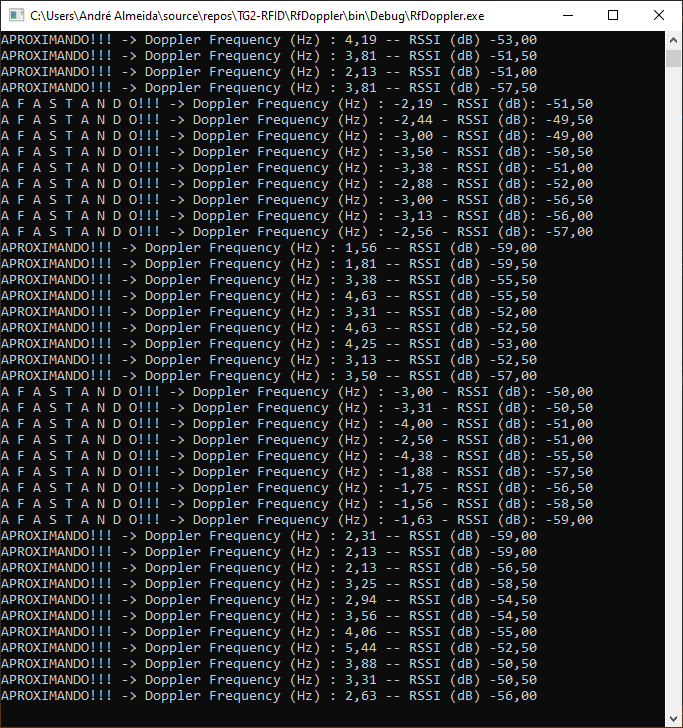
\includegraphics[width=0.8\linewidth]{figs/Metodologia/teste_doppler+RSSI_corte_60db.PNG}
    \caption{Captura de tela mostrando os dados de frequência Doppler e potência RSSI capturados no teste preliminar}
    \label{fig:teste_preliminar}
\end{figure}
 
 O teste se mostrou bastante promissor, pois é possível observar na figura \ref{fig:teste_preliminar} que realizando as configurações corretas e aplicando filtros para rejeitar \textit{outliers} de leitura é possível extrair informações úteis das leituras. Neste teste o valor da frequência Doppler foi observado para definir se a TAG se aproxima ou se afasta da antena.
 
 Ainda é possível perceber que as leituras de frequência Doppler e RSSI, seguem tendências bem definidas. As leituras de frequência Doppler são positivas ao aproximar a TAG da antena, e negativas ao afastar a TAG da antena. A transição entre leituras positivas e negativas ocorre no exato momento de passagem na frente da leitora. As leituras de potência RSSI tentem a ser maiores no momento em que a pessoa está mais próxima da antena, e menores a medida em que se afasta da antena.
 
 Apesar de seguirem uma tendência bem definida, possuem variações abruptas, algumas vezes no sentido oposto ao esperado. Por exemplo, observa-se uma queda abrupta de -51,00 dB e -52,50 dB para -57,00 dB nas duas transições entre o momento em que a pessoa se aproxima e o momento em que a pessoa se afasta da antena. Quanto ao efeito Doppler, este é proporcional à velocidade da pessoa, entretanto, o caminhar de uma pessoa não segue uma velocidade constante a todo momento, e portanto nota-se uma flutuação constante no valor lido.
